\documentclass[12pt,letterpaper]{article}

\usepackage[top=2cm,right=2cm,bottom=2cm,left=2cm,nohead,nofoot]{geometry}

\usepackage{amsmath}
\usepackage{graphicx}
\usepackage{indentfirst}
\usepackage{url}
\usepackage{mdwlist}
\usepackage[compact]{titlesec}
\usepackage[T1]{fontenc}
\usepackage{palatino}
\usepackage[brazil]{babel}
\usepackage[utf8]{inputenc}
\usepackage{enumerate}

\pagestyle{empty}
\setcounter{secnumdepth}{5}
\renewcommand{\thefootnote}{\Roman{footnote}}

\makeatletter
\def\thickhrulefill{\leavevmode \leaders \hrule height 1pt\hfill \kern \z@}
\renewcommand{\maketitle}{
	\begingroup
		\parindent \z@
		\begin{center}
			{\normalsize \@author\par}%
			\thickhrulefill\par
			{\small\raggedleft \@date\par}%
			{\Large\raggedright \@title\par}%
		\end{center}%
	\endgroup
}
\makeatother

\title{F 429: Experimento II}
\author{033910 Leandro Mendes | 104198 Thiago Verratti | 118451 Rafael Mendes | 121096 Leonardo Sorensen}
\begin{document}
\maketitle
\tableofcontents
\listoffigures
\listoftables
\newpage
\section{Introdução}
Este experimento propõe-se a estudar as experimentalmente e analizar as formas de onda dos circuitos integrador e
diferenciador. Neste caso, são do tipo RC e compostos por uma fonte, um resistor e um
capacitor ligados em série.\\
Analisamos também transientes em circuito ressonante série RLC. Os transientes podem ser estudados no laboratório excitando o circuito com uma onda quadrada de período muito maior que a constante de tempo do circuito.
\section{Instrumentos e Componentes}
Os instrumentos e componentes utilizados estão listados abaixo com seus respectivos valores nominais.
\begin{itemize}
\item{Gerador de Funções Tektronix CFG 253.} 
\item{Osciloscópio digital Tektronix TDS1000.}
\item{Resistências nominais de 47$\Omega$ e 150$\Omega$.}
\item{Resistência de décadas (10$\Omega$ a 10K$\Omega$).}
\item{Capacitor de 0.22$\mu$F.}
\item{Indutor de 50mH.}
\end{itemize}
\subsection{Medidas}
\subsubsection{Impedância interna do gerador} \label{itm:rger} Para determinar a impedância interna do gerador de funções, começamos com a aproximação de que esta é puramente resistiva e independe da frequência, modo de onda ou corrente que fornece. Feita essa hipótese, podemos encontrar a resistência interna $R_G$ do gerador montando o circuito como na figura abaixo. 
\begin{figure}[!htb]
  \centering
  \label{imgger}
  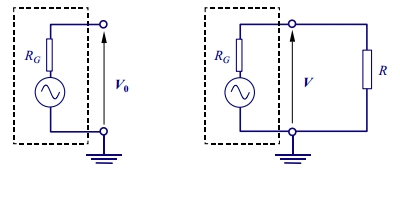
\includegraphics[scale=0.5]{impger.jpg}
  \caption{Circuito representativo para medida da resistência interna do gerador}
\end{figure}
Primeiro medimos a tensão de saída do gerador de funções conectando-o diretamente ao osciloscópio. Após medir o pico $V_0$, colocamos um resistor em paralelo ao circuito, e obtemos um valor para V. Com essas medidas podemos encontrar um valor para $R_G$, sabendo que temos um divisor de tensão e juntando a Lei de Ohm \footnote{\boxed{V = R\cdot I}}. Logo, $R_G = R \cdot (\frac{V_0}{V}-1)$ e $\Delta{R_G} = R_G \cdot \sqrt{(\frac{\Delta(\frac{V_0}{V})}{\frac{V_0}{V}-1})^2 + (\frac{\Delta{R}}{R})^2}$, onde $\Delta{\frac{V_0}{V}} = \frac{V_0}{V} \cdot \sqrt{(\frac{\Delta{V_0}}{V_0})^2 + (\frac{\Delta{V}}{V})^2}$.\\ Portanto, para \boxed{V_0 = 24,8V}\footnote{Escala: 5V}, \boxed{V = 12,2V}\footnote{Escala: 2V} e \boxed{R_{47} = 47,8\Omega , \Delta{R_{47}}=0,6\Omega}\footnote{Dado obtido no experimento I}, temos: \boxed{\Delta{V_0}=0,9940V, \Delta{V}=0,4660V}, resultando em \boxed{\frac{V_0}{V}=2,0328\frac{V}{V}, \Delta{\frac{V_0}{V}}=0,1125\frac{V}{V}} e \boxed{R_G = 49,3672\Omega \pm 5,4154\Omega}.
\subsubsection{Indutor}\label{itm:indutor} No experimento I, calculamos o valor do indutor utilizado nos experimentos. O resultado foi, \boxed{L = 47,0311mH \pm 4,0174mH}.
\subsubsection{Resistência em série do indutor ($R_L$)} \label{itm:rindutor}  O cálculo de $R_L$ foi apresentado no relatório I, resultando em \boxed{R_L = 46,3\Omega \pm 0,6\Omega}.
\subsubsection{Capacitor} \label{itm:capacitor} No experimento anterior obtivemos \boxed{C = 0,2236\mu F \pm 0,0191\mu F}.
\subsubsection{Resistor de 47$\Omega$}\label{itm:r47} \boxed{R_{47} = 47,8\Omega \pm 0,6\Omega}.
\subsubsection{Resistor de 150$\Omega$}\label{itm:r150} \boxed{R_{150} = 148\Omega \pm 2,5\Omega}.
\section{Circuito RC}
\subsubsection{Integrador}
Um circuito integrador é um componente eletrônico contendo elementos, como fonte de tensão[\ref{itm:rger}], resistor[\ref{itm:r150}] e capacitor[\ref{itm:capacitor}].
\begin{figure}[!htb]
  \centering
  \label{imgint}
  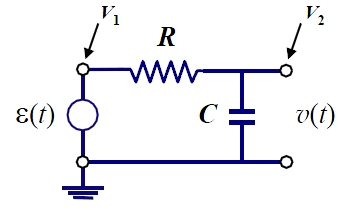
\includegraphics[scale=0.5]{integrador.jpg}
  \caption{Circuito integrador ou Filtro passa-baixa}
\end{figure}
\begin{enumerate}[I]
\item \textbf{Lei de Kirchoff}: Aplicando a lei de Kirchoff para malhas teremos: $\varepsilon(t) = R\cdot i(t) + v_c(t)$\footnote{Lembrando que \boxed{I_c(t) = C \cdot \frac{\mathrm d V(t)}{\mathrm d t}}}
\item \textbf{Integrador}: No cálculo acima obtemos: $v(t)\approx v_0(t) + \frac{1}{RC} \int_{t_0}^{t} \varepsilon(t)dt.$
\item \label{itm:passabaixa} \textbf{Passa-baixa}: A função de transferência de um passa-baixa\footnote{Sedra Smith, microeletronics circuits 5th edition , tabela 1.2: Resposta em frequência de redes STC} é dada por $T(s) = \frac{K}{1 + \frac{s}{w_0}}$.\\
  Sabe-se que $s = j \cdot w$, onde $w = 2\pi \cdot f$ e $\tau = \frac{1}{w_0}$\footnote{frequência 3-dB}.\\
Portanto, para um passa-baixa temos: $T(jw) = \frac{K}{1 + j(\frac{w}{w_0})}$ e a frequência de corte $f_c = \frac{1}{\tau \cdot 2\pi}$.
\subitem \label{itm:intdc} \textbf{Transmissão DC}: Em uma transmisao DC, ou seja, $f = 0Hz (w = 0)$, temos $T(jw) = K$.
\item \textbf{Metodologia}: Montamos o circuito conforme a figura acima, monitorando a $V_1$ e $V_2$ no osciloscópio, variando as formas de onda\footnote{quadrada, triângular e senoíde} e a frequência ( $\frac{f_c}{40}$ , $f_c$, $40f_c$ ). Modificamos, também, o nível DC entre -1V e +1V e observamos o efeito provocado.
\item \label{itm:intred} \textbf{Resultados}: Dado em \ref{itm:passabaixa}, combinando com \ref{itm:capacitor} e \ref{itm:r150}, temos $f_c \approx 4,8881Hz$.
\begin{figure}[!htb]
  \centering
  \label{fd40int}
  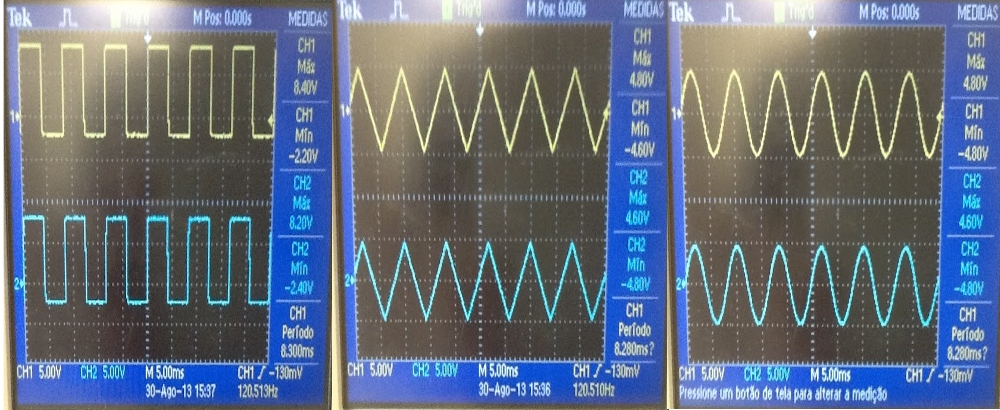
\includegraphics[scale=0.52]{img/fd40int.jpg}
  \caption{Circuito integrador $f_c \approx 120,51Hz$}
\end{figure}
\begin{figure}[!htb]
  \centering
  \label{fint}
  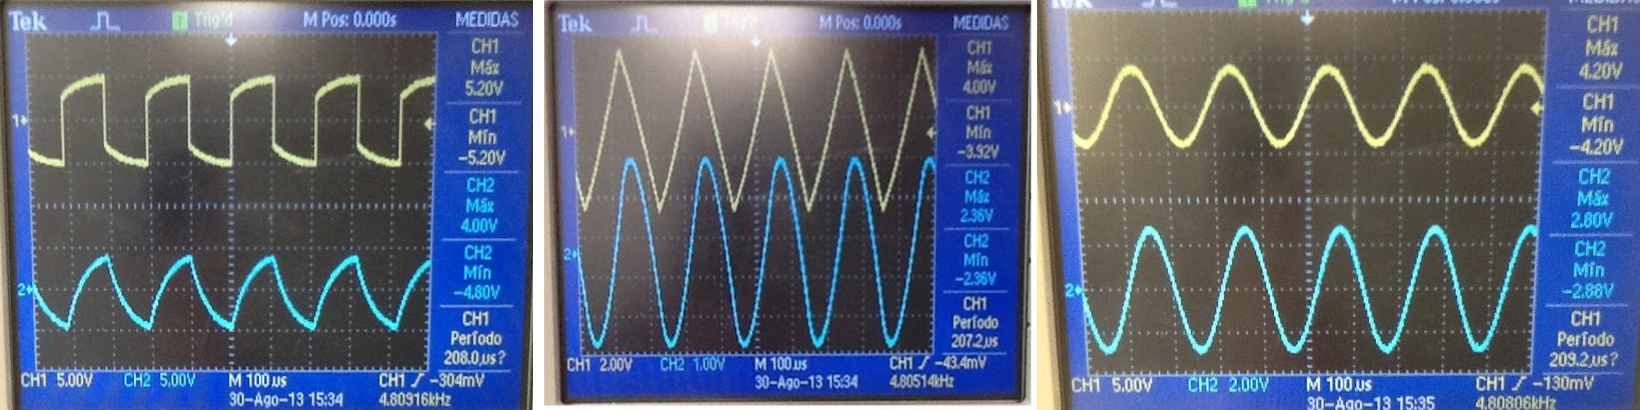
\includegraphics[scale=0.32]{img/fint.jpg}
  \caption{Circuito integrador $f_c$}
\end{figure}
\begin{figure}[!htb]
  \centering
  \label{f40int}
  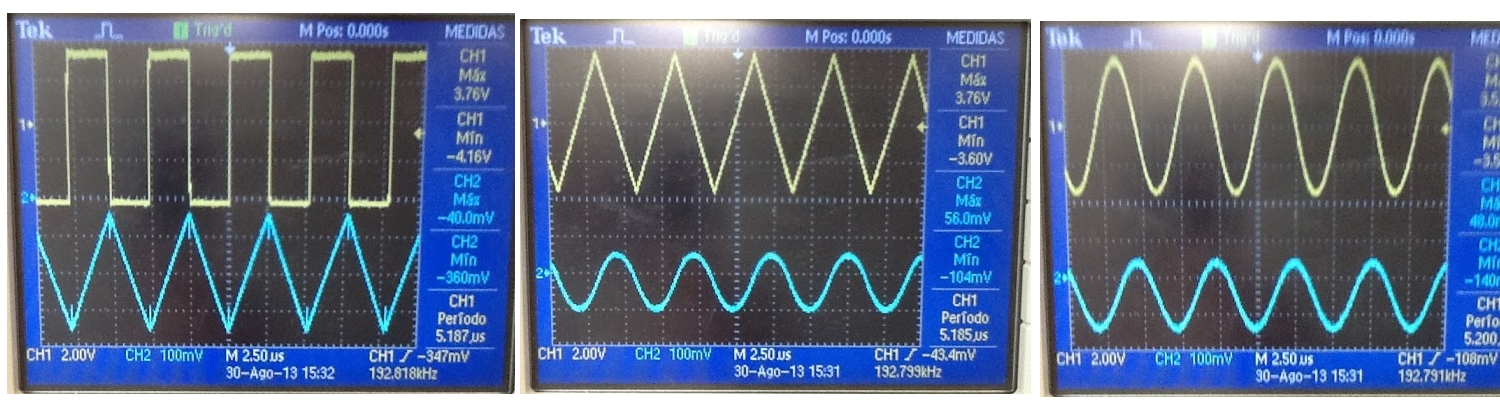
\includegraphics[scale=0.35]{img/f40int.jpg}
  \caption{Circuito integrador $f_c \approx 192,80kHz$}
\end{figure}
Para \ref{fd40int}, ou seja, frequências aquém de $f_c$, temos que $V_1 \approx V_2$ visto que o circuito é um passa-baixa[\ref{itm:passabaixa}]\footnote{Nota-se no diagrama de Bode do experimento I para um circuito RC}. Entretanto, para frequência próximas de $f_c$ observamos pequenas distorções em $V_2$ e para frequência muito além ($40f_c$) temos um integrador, visto que, a integral de uma constante é uma reta. \\
A variação do sinal DC resultou em uma descida/subida mais abrupta, já que teremos $T(jw) = K = 1, para f = 0$.
\end{enumerate}
\subsubsection{Diferenciador}
O circuito RC diferenciador assemelha-se ao integrador, apenas alteramos a configuração entre o resistor \ref{itm:r150} e o capacitor \ref{itm:capacitor}.
\begin{figure}[!htb]
  \centering
  \label{imgint}
  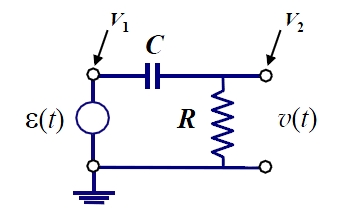
\includegraphics[scale=0.5]{diferenciador.jpg}
  \caption{Circuito diferenciador ou Filtro passa-alta}
\end{figure}
\begin{enumerate}[I]
\item \textbf{Lei de Kirchoff}: Aplicando a lei de Kirchoff para malhas teremos: $\varepsilon(t) = \frac{t}{C} + v(t)$.
\item \textbf{Diferenciador}: No cálculo acima obtemos: $v(t) \approx \frac{1}{RC}\frac{d\varepsilon(t)}{dt}$
\item \label{itm:passaalta} \textbf{Passa-alta}: A função de transferência de um passa-alta\footnote{Sedra Smith, microeletronics circuits 5th edition , tabela 1.2: Resposta em frequência de redes STC} é dada por $T(s) = \frac{Ks}{s + w_0}$.\\
  Sabe-se que $s = j \cdot w$, onde $w = 2\pi \cdot f$ e $\tau = \frac{1}{w_0}$\footnote{frequência 3-dB}.\\
Portanto, para um passa-alta temos: $T(jw) = \frac{K}{1 - j(\frac{w_0}{w})}$ e a frequência de corte $f_c = \frac{1}{\tau \cdot 2\pi}$.
\subitem \label{itm:intdc} \textbf{Transmissão DC}: Em uma transmisao DC, ou seja, $f = 0Hz (w = 0)$, temos $T(jw) = 0$.
\item \textbf{Metodologia}: Montamos o circuito conforme a figura acima, monitorando a $V_1$ e $V_2$ no osciloscópio, variando as formas de onda\footnote{quadrada, triângular e senoíde} e a frequência ( $\frac{f_c}{40}$ , $f_c$, $40f_c$ ). Modificamos, também, o nível DC entre -1V e +1V e observamos o efeito provocado.
\item \label{itm:intred} \textbf{Resultados}: Dado para um filtro passa-alta \ref{itm:passaalta}, combinando com o capacitor \ref{itm:capacitor} e resistor \ref{itm:r150}, temos:
\begin{figure}[!htb]
  \centering
  \label{fd40d}
  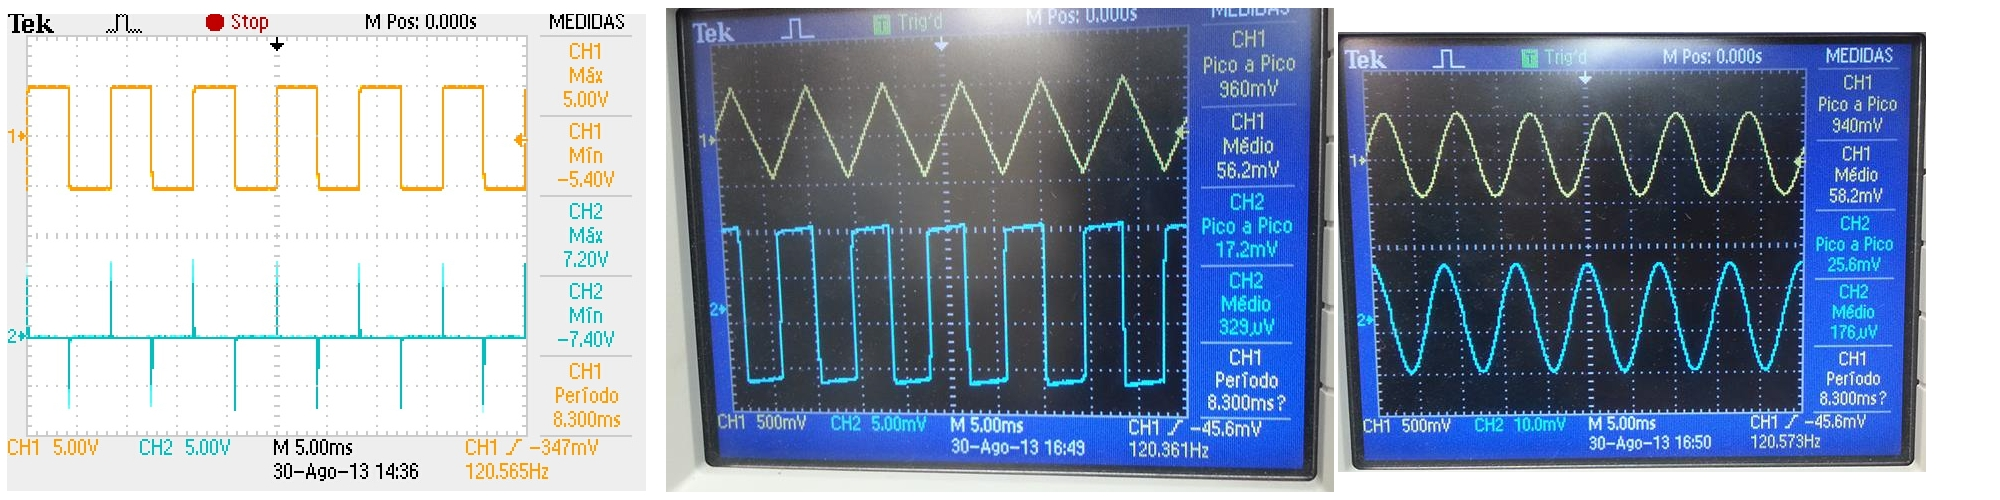
\includegraphics[scale=0.62]{img/fd40d.jpg}
  \caption{Circuito diferenciador $f_c \approx 120,51Hz$}
\end{figure}
\begin{figure}[!htb]
  \centering
  \label{fd}
  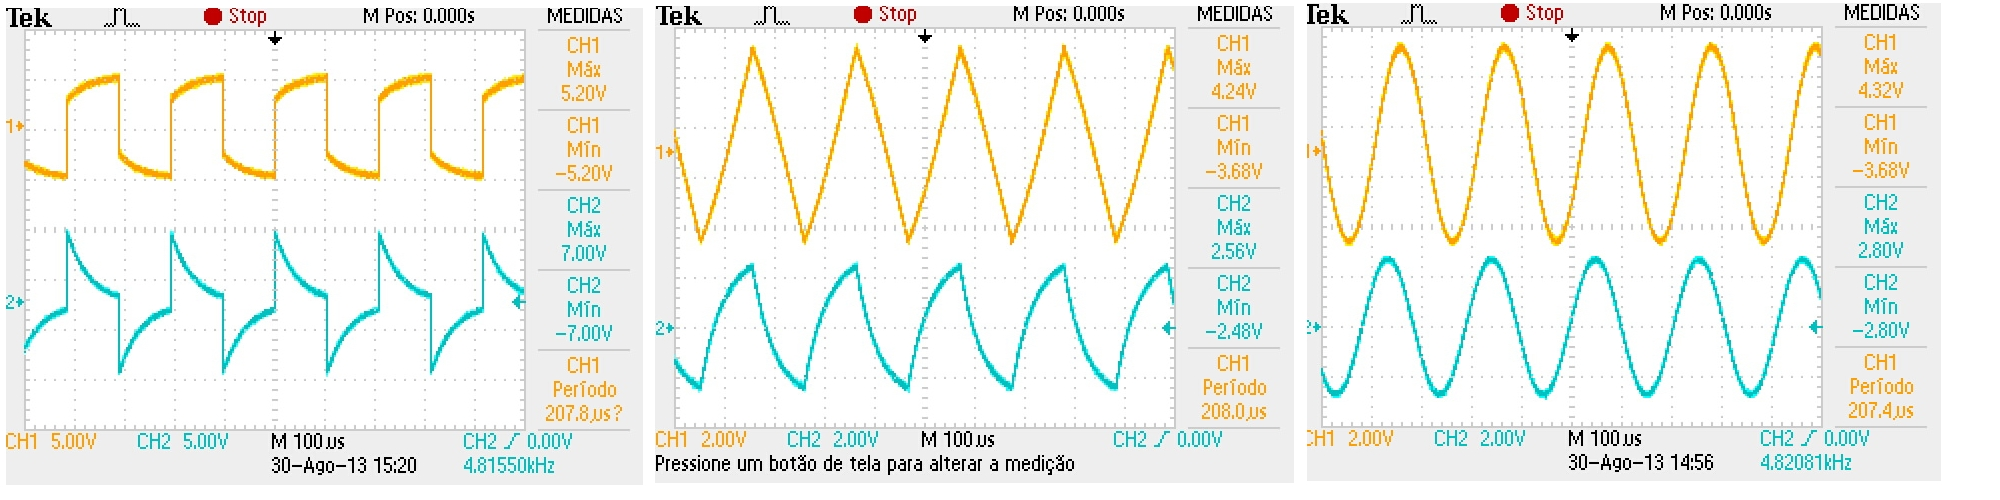
\includegraphics[scale=0.62]{img/fd.jpg}
  \caption{Circuito diferenciador $f_c$}
\end{figure}
\begin{figure}[!htb]
  \centering
  \label{f40d}
  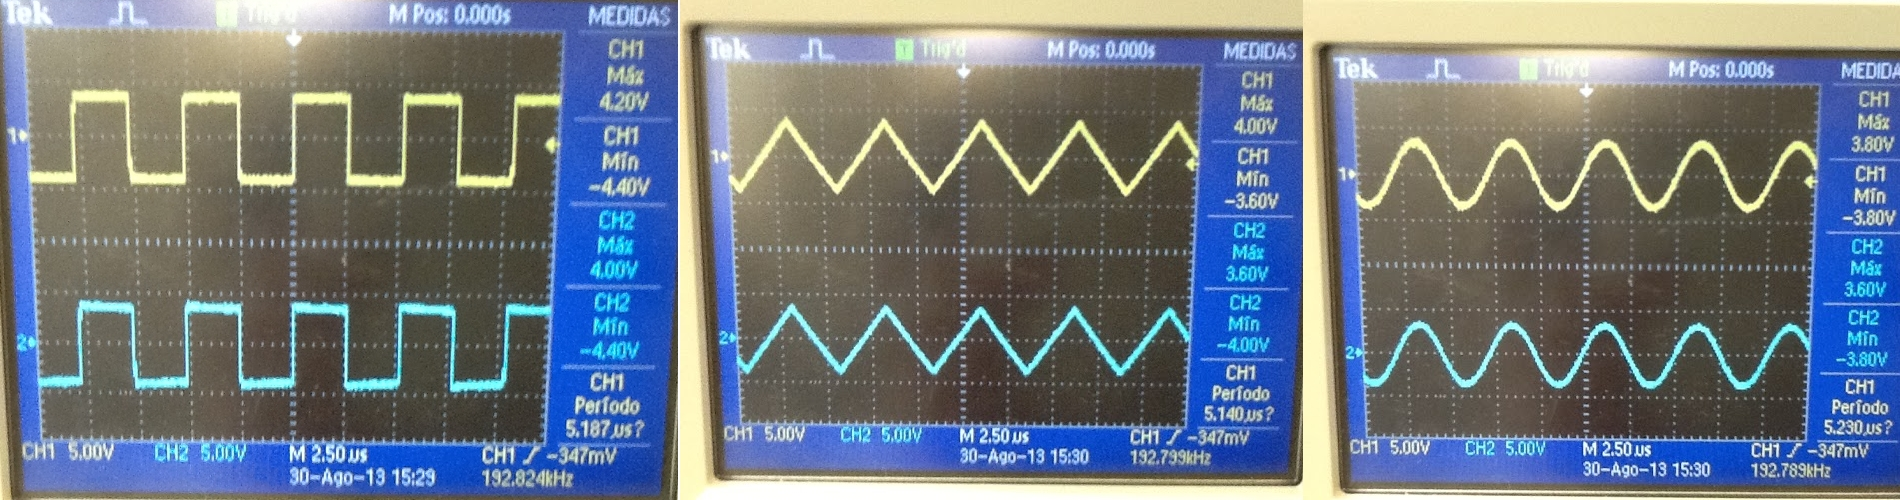
\includegraphics[scale=0.25]{img/f40d.jpg}
  \caption{Circuito diferenciador $f_c \approx 192,80kHz$}
\end{figure}
Para \ref{fd40d}, ou seja, frequências aquém de $f_c$, temos um circuito integrador, conforme observado na figura \ref{fd40d}, na qual para a onda triângular, fica claro que, a derivada de uma reta é uma constante. Já para frequência bem próxima a $f_c$ temos uma distorção na saída, e para $f >> f_c, ou seja, f \approx 40f_c$ temos $V_1 \approx V_2$, visto que temos um filtro passa-alta. 
A variação do sinal DC não modificou a saída $V_2$, uma vez que, o capacitor carrega-se rápidamente em tensão/corrente DC e, diferentemente de uma onda variável no tempo, o capacitor não se descarregará.
\end{enumerate}
\end{document}


